\documentclass{article}
\usepackage{amsmath}
\usepackage{bm}
\usepackage[pdftex]{graphicx,color}

\textwidth 6in
\oddsidemargin 0.25in
\textheight 9in
\topmargin 0in
\headsep 0in

\parindent 12pt
\parskip 12pt

\renewcommand{\vec}[1]{\bm{#1}}
\newcommand{\nbar}{\bar{n}}

\title{Analytic KL mode calculation for thin spherical shell}
\date{}
\begin{document}
\maketitle

We wish to compute the signal-to-noise eigenmodes and eigenvalues explicitly
for the case where our survey geometry is a thin spherical shell of thickness
$\epsilon$, at radial distance $R$, with constant number density $\nbar_0$
within the shell, and where our two-point correlation function is homogeneous
and isotropic (i.e., in real space) with the functional form $\xi(r) = A e^{-br^2}$.
To recall, the signal and noise contributions to the covariance of the pixels
$x_i = \int d^3x~ \psi_i(\vec{x}) n(\vec{x})$ are given by
\begin{align}
    S_{ij} &= \int d^3x_1 \int d^3x_2~ \psi_i^*(\vec{x}_1) \psi_j(\vec{x}_2) \nbar(\vec{x}_1) \nbar(\vec{x}_2) \xi(\vec{x}_1, \vec{x}_2), \\
    N_{ij} &= \int d^3x~ \psi_i^*(\vec{x}) \psi_j(\vec{x}) \nbar(\vec{x}).
\end{align}

We first show that, for a very thin shell, the eigenmodes are simply
proportional to spherical harmonic functions,
$\psi_i(\vec{x}) = C_i Y_\ell^m(\hat{x})$.
To see this, first note that the noise matrix is already diagonal for this
choice of $\psi_i$, owing to the orthogonality of spherical harmonics:
\begin{equation}
    N_{ij} = \int_R^{R+\epsilon} r^2 dr \int d\Omega_{\hat{x}}~ C_i^* Y_\ell^{m*}(\hat{x}) ~ C_j Y_{l'}^{m'}(\hat{x}) ~ \nbar_0
           = R^2 \epsilon \nbar_0~ |C_i|^2 \delta_{ij}.
\end{equation}
(Here and in the following, we treat $i$ and $j$ as double indices, with
$i = \ell m$ and $j = \ell' m'$.)

The signal-to-noise eigenmodes are therefore just the functions that make the
signal matrix diagonal.  Since the correlation function is homogeneous and we
are dealing with a thin shell, we have
\begin{equation}
    \xi(\vec{x}_1,\vec{x}_2) = \xi(|R\hat{x}_1-R\hat{x}_2|) = \xi\left(R\sqrt{2(1-\hat{x}_1\cdot\hat{x}_2}\right).
%    = A e^{-2bR^2(1-\hat{x}_1\cdot\hat{x}_2)}.
\end{equation}
Importantly, this function depends only on the dot product of the two direction
vectors, $\hat{x}_1\cdot\hat{x}_2$.  It can therefore be expanded as a sum of
Legendre polynomials,
$\xi(\vec{x}_1,\vec{x}_2) = \sum_\ell a_\ell P_\ell(\hat{x}_1\cdot\hat{x}_2)$
for some real coefficients $a_\ell$.  Using the identity
\begin{equation}
    P_\ell(\hat{x}_1\cdot\hat{x}_2) = \frac{4\pi}{2\ell+1} \sum_{m=-\ell}^\ell Y_\ell^m(\hat{x}_1) Y_\ell^{m*}(\hat{x}_2),
\end{equation}
we see that the signal matrix
\begin{align}
    S_{ij} &= \int_R^{R+\epsilon} r_1^2 dr_1 \int d\Omega_{\hat{x}_1} \int_R^{R+\epsilon} r_2^2 dr_2 \int d\Omega_{\hat{x}_2} ~ C_i^* Y_\ell^{m*}(\hat{x}_1) ~ C_j Y_{\ell'}^{m'}(\hat{x}_2) ~ \nbar_0^2 \\
           &\quad \times \sum_{\ell'',m''} a_{\ell''} \frac{4\pi}{2\ell''+1} Y_{\ell''}^{m''}(\hat{x}_1) Y_{\ell''}^{m''*}(\hat{x}_2) \\
           &= R^4 \epsilon^2 \nbar_0^2 ~ a_\ell \frac{4\pi}{2\ell+1} |C_i|^2 \delta_{ij},
\end{align}
is indeed diagonal, again owing to the orthogonality of spherical harmonics.

For convenience we choose the normalization constant $C_i$ so as to make the
noise matrix precisely equal to the identity matrix, i.e.,
$C_i = (R^2 \epsilon \nbar_0)^{-1/2}$.  Then $N_{ij} = \delta_{ij}$ and
\begin{equation}
    S_{ij} = 4\pi R^2 \epsilon \nbar_0 ~ \frac{a_\ell}{2\ell+1} ~ \delta_{ij}.
\end{equation}
Note that the eigenvalues $\lambda_i = S_{ii}$ are independent of $m$.  This
gives us the freedom to choose our eigenmodes to be real-valued functions, by
taking appropriate combinations of $Y_\ell^m$'s.  Specifically we define real
spherical harmonics by
\begin{equation}
    Y_{\ell m} =
    \begin{cases}
        Y_\ell^0 & \text{if } m = 0, \\
        \frac{1}{\sqrt{2}} (Y_\ell^m + (-1)^m Y_\ell^{-m}) \propto P_\ell^m(\cos\theta) \cos m\phi & \text{if } m > 0, \\
        \frac{1}{i\sqrt{2}} (Y_\ell^{-m} - (-1)^m Y_\ell^m) \propto P_\ell^m(\cos\theta) \sin m\phi & \text{if } m < 0,
    \end{cases}
\end{equation}
and choose our eigenmodes to be $\psi_i = (R^2\epsilon \nbar_0)^{-1/2} Y_{\ell m}$.

Thus far we have seen that, so long as the two-point correlation function
depends only on the directional dot product $\hat{x}_1\cdot\hat{x}_2$, the
signal-to-noise eigenmodes can be taken to be real spherical harmonics.  To
compute the eigenvalues we need to consider the specific form of the
correlation function, which we take to be $\xi(r) = A e^{-br^2}$, or
\begin{equation}
    \xi(\vec{x}_1,\vec{x}_2)
        = A e^{-b|\vec{x}_1-\vec{x}_2|^2}
        = A e^{-2bR^2(1 - \hat{x}_1\cdot\hat{x}_2)}
        = A e^{-y} e^{y (\hat{x}_1\cdot\hat{x}_2)},
\end{equation}
where we define $y \equiv 2bR^2$ for convenience.  After Taylor-expanding
the exponential and using the identity
\footnote{\texttt{http://mathworld.wolfram.com/LegendrePolynomial.html}}
\begin{equation}
    x^n = \sum_{\ell=n,n-2,\dots} \frac{(2\ell+1) n!}{2^{(n-\ell)/2} \left(\frac{1}{2}(n-\ell)\right)! (\ell+n+1)!!} P_\ell(x),
\end{equation}
we have
\begin{align}
    e^{y(\hat{x}_1\cdot\hat{x}_2)}
        &= \sum_{n=0}^\infty \frac{y^n}{n!} \sum_{\ell=n,n-2,\dots} \frac{(2\ell+1) n!}{2^{(n-\ell)/2} \left(\frac{1}{2}(n-\ell)\right)! (\ell+n+1)!!} P_\ell(\hat{x}_1\cdot\hat{x}_2) \\
        &= \sum_{\ell=0}^\infty \left( \sum_{n=\ell,\ell+2,\dots} \frac{y^n}{n!} \frac{(2\ell+1) n!}{2^{(n-\ell)/2} \left(\frac{1}{2}(n-\ell)\right)! (\ell+n+1)!!} \right) P_\ell(\hat{x}_1\cdot\hat{x}_2) \\
        &= \sum_{\ell=0}^\infty \left( \sum_{k=0}^\infty y^{\ell+2k} \frac{(2\ell+1)}{2^k k! (2\ell+2k+1)!!} \right) P_\ell(\hat{x}_1\cdot\hat{x}_2).
\end{align}
The coefficients of the Legendre expansion
$\xi(\vec{x}_1,\vec{x}_2) = \sum_\ell a_\ell P_\ell(\hat{x}_1\cdot\hat{x}_2)$
are therefore
\begin{equation}
    a_\ell = A e^{-y} \sum_{k=0}^\infty y^{\ell+2k} \frac{(2\ell+1)}{2^k k! (2\ell+2k+1)!!},
\end{equation}
which gives us for the signal-to-noise eigenvalues
\begin{equation}
    \lambda_i = S_{ii} = 4\pi R^2 \epsilon \nbar_0 ~ A e^{-y} \sum_{k=0}^\infty \frac{y^{\ell+2k}}{2^k k! (2\ell+2k+1)!!}.
\end{equation}
Note that the factor $4\pi R^2\epsilon \nbar_0$ is just the expected number
of galaxies in the shell.  The function
$f_\ell(y) = e^{-y} \sum_k \frac{y^{\ell+2k}}{2^k k! (2\ell+2k+1)!!}$
is plotted in the upper panel of Figure \ref{fig:fly} for $0 \le \ell \le 5$.
For $\ell = 0$ the series evaluates to $f_0(y) = y^{-1} e^{-y} \sinh y$, which
decays asymptotically as $1/(2y)$.  The lower panel of Figure \ref{fig:fly}
shows that, in fact, all the $f_\ell$'s have the same asymptotic behavior.

\begin{figure}
\begin{center}
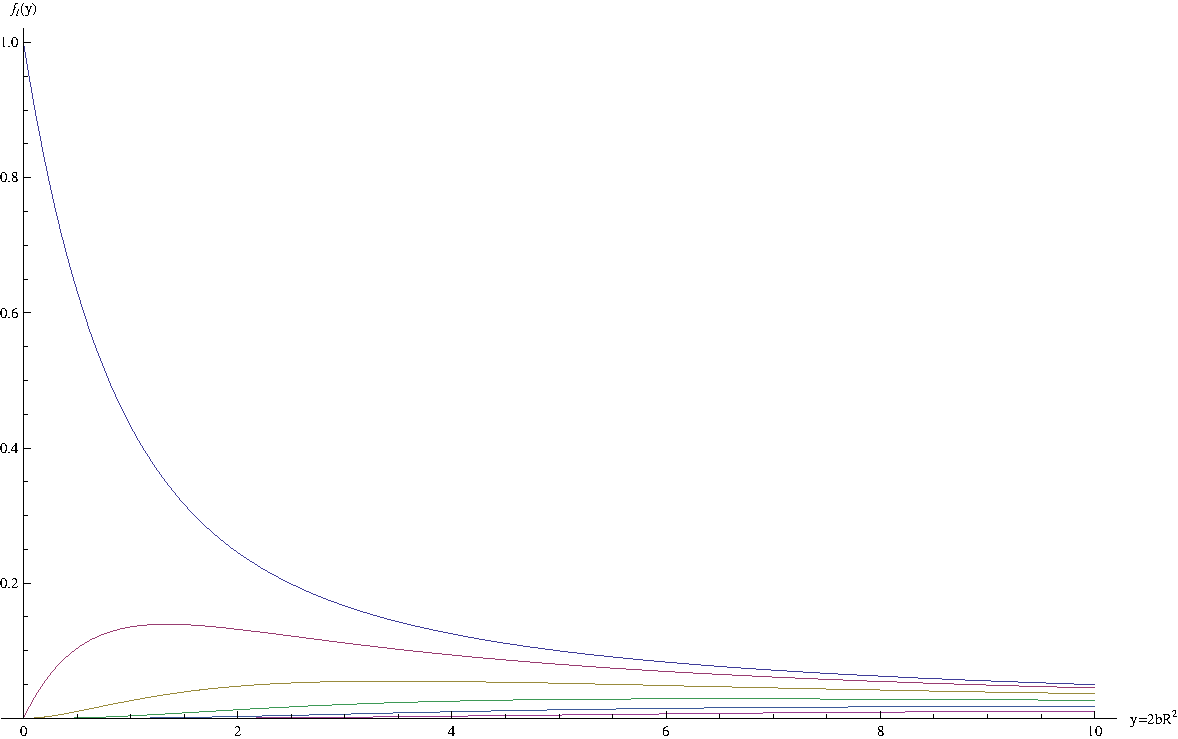
\includegraphics[width=\textwidth]{fly}
\end{center}
\begin{center}
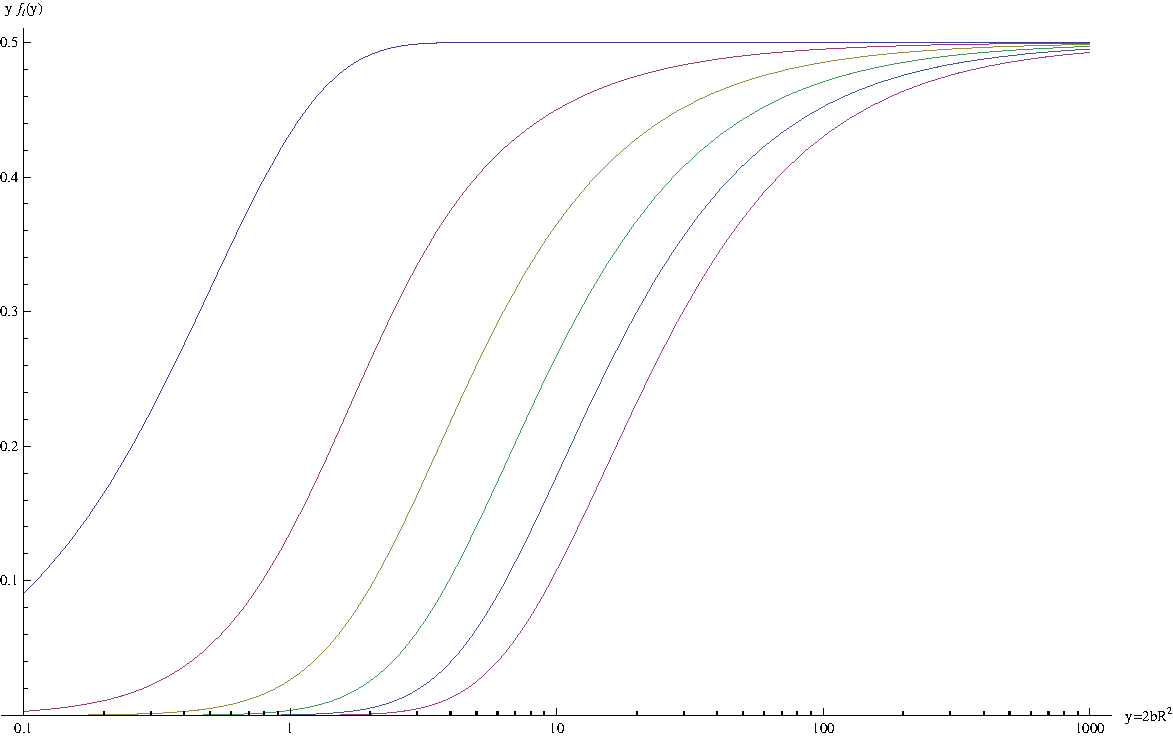
\includegraphics[width=\textwidth]{logfly}
\end{center}
\caption{(Upper panel) The function
$f_\ell(y) = e^{-y} \sum_{k=0}^\infty \frac{y^{\ell+2k}}{2^k k! (2\ell+2k+1)!!}$
plotted for $\ell = 0$ (top-most curve) to $\ell = 5$ (bottom-most curve).
(Lower panel) The function $y f_\ell(y)$, showing that asymptotically
$f_\ell(y) \sim 1/(2y)$.}
\label{fig:fly}
\end{figure}

\end{document}
